\documentclass[12pt]{report}
\usepackage{graphicx}
\usepackage{float}
\usepackage{lettrine}
\usepackage{caption}
\usepackage{url}
\usepackage[margin=1in]{geometry}
\usepackage{amsmath}
\usepackage{algorithm}
\usepackage[noend]{algpseudocode}
\usepackage{amssymb}

\newcommand\blfootnote[1]{%
  \begingroup
  \renewcommand\thefootnote{}\footnote{#1}%
  \addtocounter{footnote}{-1}%
  \endgroup
}

\title{Verification of Sequential Elliptic Curve Arithmetic Circuits Using Algebraic Geometry}
\author{Jaden Simon - simonjaden223@gmail.com \\ \and
	   Daniel Humeniuk - d.humeniuk@utah.edu}

	   
\begin{document}

\maketitle

\section{Introduction}

For our term project in ECE 5745, we intend to perform verification of point-scalar multiplication over an ellitpic curve. The design we are working with relies on a scalar and point (two evenly sized $x$ and $y$ coordinates) over two busses and multiplied over an arbitrary elliptical curve using modular arithmetic. The design relies on sequential logic so we will be using some techniques from \cite{Kalla} to traverse the circuit.

We will be studying a 3-bit ECC circuit as a proof of concept. ECC relies on a much larger bit count for security, but for time's sake we are verifying a much smaller circuit. For an $n$-bit ECC circuit, we can perform arithmetic over $\mathbb{F}_{2^n}$, which would be a binary elliptic curve. In software, the field is generally $\mathbb{F}_{p}$ where $p$ is a prime number. Such a field is difficult to work on with hardware, so for this project we will focus exclusively on binary elliptic curves. Note that $n$ is ideally a prime number, otherwise a composite field is formed and mathematical techniques can be used to exploit vulnerabilities in the design. 

Arithmetic over fields of $2^n$ is relatively straightforward. Addition is simply bitwise XOR, multiplication can be done with Mastrovito or Montogomery multipliers, and division can be done by finding the inverse using the extended GCD algorithm. GCD will be computed using the binary GCD algorithm, for which a generic circuit implementation can be found in Figure \ref{fig:gcd}. The inverter circuit has additional accumalators that are not shown. With these basic functions implemented as circuits, we can first create a point-adder. The point-adder will compute the slope $m$ between two points $(x1, y1), (x2, y2)$, then output a new point using the formulas: $x = m^2 + x1 + x2$ and $y = m(x1 + x) + y1$. Point-scalar multiplication can then be done using repeated point addition. If time allows, we will create a more sophisticated circuit using point doubling and attempt to verify that as well. For the point-adder and GCD circuits we will need sequential-circuit verification techniques. 

\begin{figure}
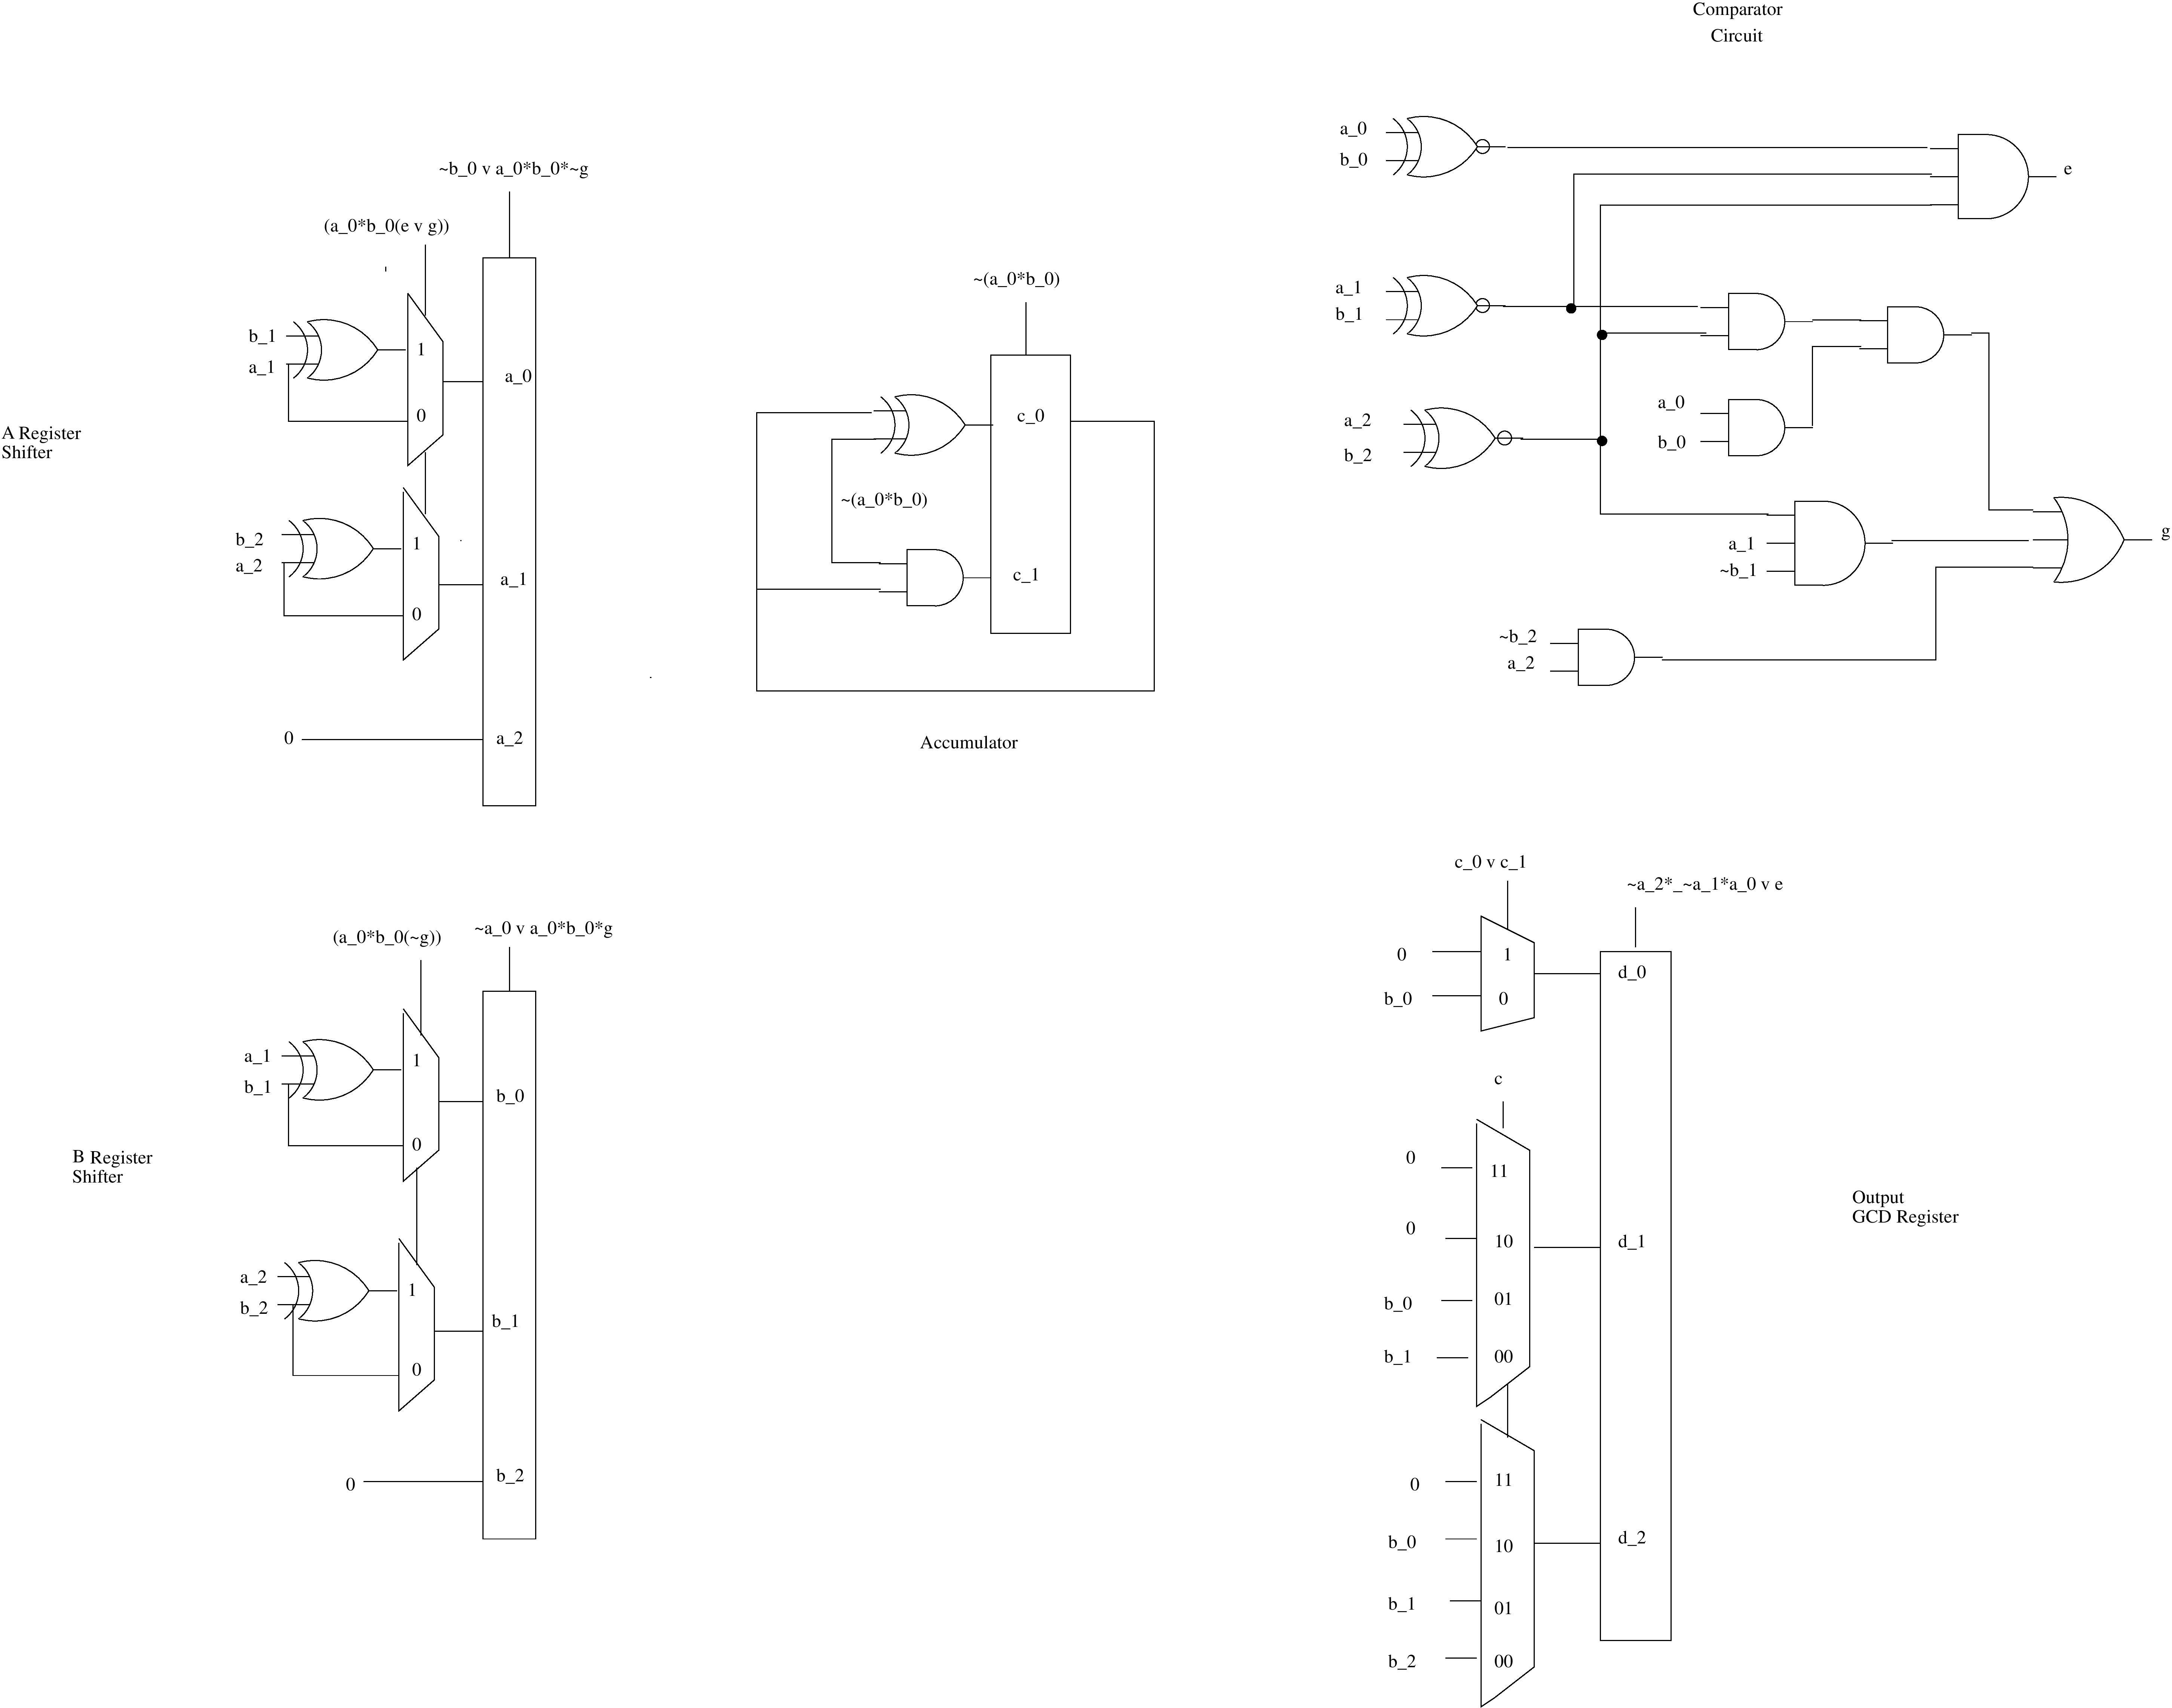
\includegraphics[scale=0.35]{images/gcd_page.png}
\caption{Binary GCD Algorithm for $3$ bits}
\label{fig:gcd}
\end{figure}

\section{Our Starting Point}

To begin, we will implement an algebraic geometry based algorithm to implicitly unroll our circuit. The algorithm can be found in \cite{Kalla} and uses projections of varieties to give next state variables in terms of present state variables. Note that our GCD circuit will always terminate after $2n$ cycles, thus for a 3-bit circuit we will require 8 cycles. Galois field multiplication will always terminate after $n$ cycles, though for our case we will use a combinational Mastrovito multiplier so it will only take 1 cycle. A full point-scalar multiplier would require $4n^2$ clock cycles. Clearly we can see that as we continue to scale up the ECC circuit, the number of iterations required grows quite rapidly. To verify the large circuits presently used some method of reducing this complexity is required, perhaps by verifying modules individualing then substituting abstractions for full analysis. 

For efficient analysis of circuits, we will need a specific term ordering. The ordering RATO as described in \cite{Kalla} places all bit-level varaibles using a reverse topological order from the circuit first, then word-level next-state outputs, then word-level present-state outputs. The Gr{\"o}bner basis can then be computed after adding the vanishing polynomials to the ideal. For our project, we then only need to derive the polynomials from our circuit, then apply RATO, and finally use Singular to compute the Gr{\"o}bner basis iteratively. The final Gr{\"o}bner basis will contain a polynomial containing only the word-level output with the word-level inputs, which we can then compare to our specification. For the inverter circuit, our spec will just be $R' + 1/A_{init}$ where $R'$ is the next-state result variable, and $A_{init}$, $B_{init}$ are the initial $A$ and $B$ input variables. For the multiplier circuit, our spec is $R' + A_{init}B_{init}$ which \cite{Kalla} already shows the verification of as a proof-of-concept. 

The specification for the standard GCD circuit in Figure \ref{fig:gcd} has yet to be determined. We will attempt to mine the specification from our above circuit using a similar technique. After that is done, we can move forward with verifying the remaning parts of point-scalar multiplier. For the point-adder and point-multiplier, we may have to define two output word-level variables, one for each coordinate, then apply the above algorithm. This should produce an output resembling the equations from the introduction: $X = ((X2 + X2)/(Y1+Y1))^2 + X1 + X2$ and $Y = ((X2 + X2)/(Y1 + Y1))(X1 + X) + Y1$. Where $X$ and $Y$ are the final next-state result variables and $X1, X2, Y1, Y2$ are the initial input variables. 

A specification polynomial for the point-multiplier would be an unrolled form of the point-adder, where the previously added point should be substituted into the same equation. The resuling specification will look quite messy, though we should still be able to verify the final circuit.

\iffalse % Not doing this algorithm 
\begin{algorithm}
\caption{Algebraic Geometry based FSM Traversal}
{\textbf{Input:} The circuit's characteristic polynomial ideal $J_{ckt}$, initial state polynomial $\mathcal{F}(S)$, and LEX term order: bit-level variables $x,s,t >$ PS word S $>$ NS word $T$}
{$from^0=reached=\mathcal{F}(S)$}
{\textbf{Do:}}
\hspace*{6mm}{$i \leftarrow i + 1 $}
\hspace*{6mm}{$G \leftarrow GB(J_{ckt}, J_{v}, from^{i-1}) $}
\hspace*{6mm}{$to^i \leftarrow G \cap \mathbb{F}_{2^k}[T]$}
\hspace*{6mm}{$new^i \leftarrow to^i + (T^{2^k} - T) : reached$}
\hspace*{6mm}{$reached \leftarrow reached*new^i$}
\hspace*{6mm}{$from^i \leftarrow new^i(S$/$T)$}
{\textbf{While:} $new^i != 1$}
{\textbf{Return:} $reached$}

\end{algorithm}

This algorithm will provide us with the the representation of the reached states in every step which we can then over $\mathcal{F}_2^k$. The variables $from$, $reached$, $to$, and $new$ represent the functions of sets in the states.
This algorithm will provide us with the the representation of the reached states in every step which we can then over $\mathbb{F}_{2^k}$. The algorithm uses the Gr\{"o}bner basis of the ideal $J$ and the vanishing ideal $J_0$. This Gr\{"o}bner basis will be used to denote the set of next states in the FSM. 

\fi



\section{Conclusion}
We have completed RTL of all components of a point-scalar multiplier and have designed a circuit schematic for a standard 3-bit GCD circuit. Our first task will be to apply the sequential circuit verification to the GCD circuit to make sure we understand what is happening and that we can apply the algorithm correctly. Next, we will create the point adder circuit and verify that. Then we will need to expand the point-adder specification to show repeated addiction to give us a specification for point-scalar multiplication. The final step would of course be verifying the functionality of a full point-scalar multiplier with all internal circuitry exposed. Of course if we have to, we can just replace components of the full circuit with our previously found specifications. This would still be a formal proof of an elliptic curve arithmetic circuit, just not with all internal circuitry exposed. 

\bibliographystyle{IEEEtran}
\bibliography{IEEEabrv,bib/ref}

\end{document}